\chapter{Realizability}
\label{chap:realizability}

\section{The basic idea}
\label{sec:realizability-basic-idea}

Given a mathematical structure (constants, functions, relations, and
axioms), what should a computer implementation look like? For simple
cases, the answer is obvious. A group would have a type whose values
represent group elements, a value representing the neutral element,
and functions which compute the group operation and inverses. But for
more interesting structures, especially those arising in mathematical
analysis, the answer is less clear. How do we implement the real
numbers (and we do not mean floating-point arithmetic, we mean the
\emph{real} real numbers)? Which operations on a compact metric space
can be implemented? How do we implement a space of smooth functions?
Significant research goes into finding satisfactory answers to such
questions~\cite{Wei00,TZ98,Bla97}.

To explain the basic idea behind realizability we consider a small
real-world programming example. Suppose we are asked to design a data
structure for the set $\mathcal{G}$ of all finite
simple\footnote{Simple means at most one arrow between any two
  vertices.} directed graphs with vertices labeled by distinct
integers. An exemplar directed graph~$G$ is shown in
Figure~\ref{fig:digraph}.
%
\begin{figure}[htp]
  \centering
  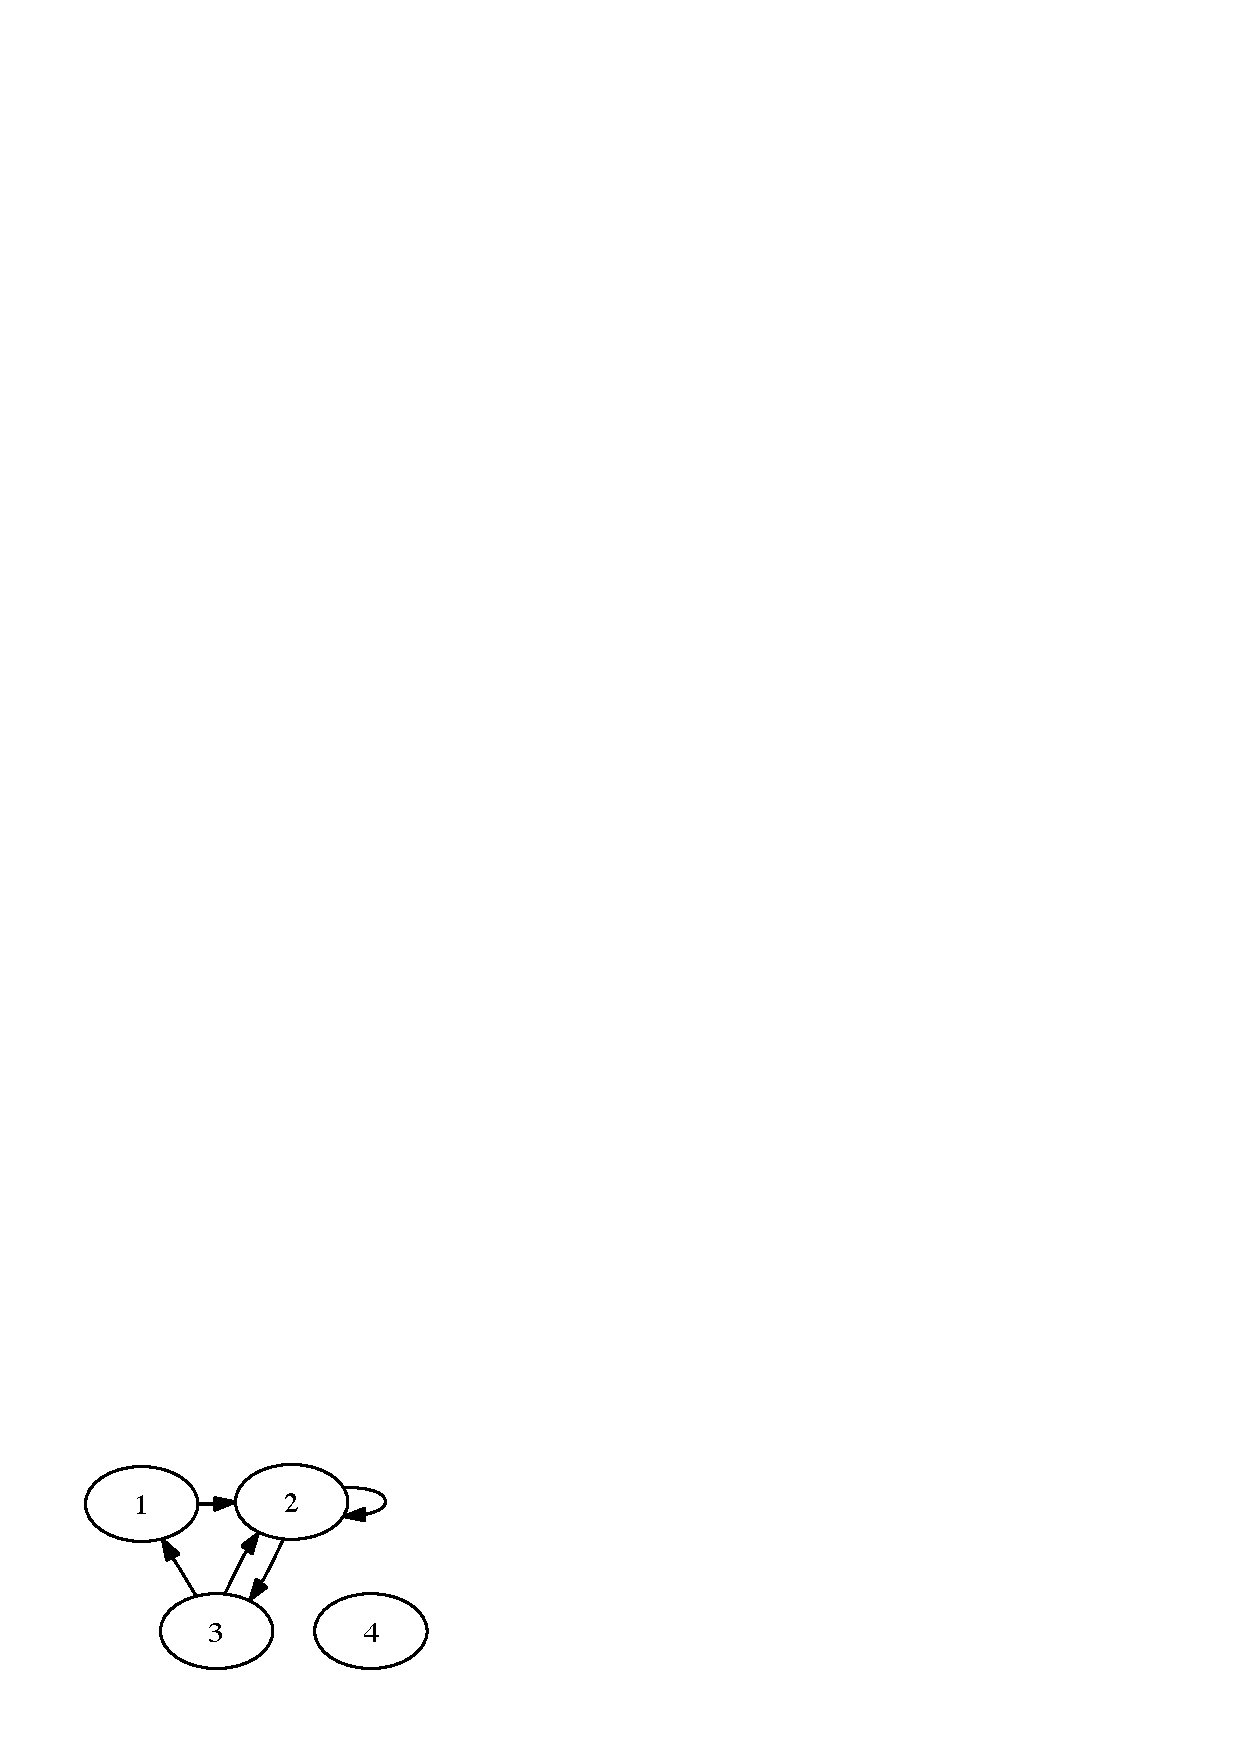
\includegraphics[width=0.3\textwidth]{digraph}
  \caption{A finite directed graph $G$}
  \label{fig:digraph}
\end{figure}
%
One common representation of such graphs uses a pair of lists
$(\ell_V, \ell_A)$, where $\ell_V$ is the list of vertex labels and
$\ell_A$ is the \emph{adjacency list} representing the arrows by
pairing the labels of each source and target. For the above graph $G$,
$\ell_V = [1, 2, 3, 4]$ and $\ell_A = [(1,2), (2,2), (2,3), (3,2),
(3,1)]$.
%
Thus we define the datatype of graphs as\footnote{We use Haskell
  notation in which $[t]$ is the type of lists of elements of
  type~$t$, and $(t_1, t_2)$ is the cartesian product of types~$t_1$
  and~$t_2$.}
%
\begin{lstlisting}[language=Haskell]
type Graph = ([Int], [(Int, Int)])
\end{lstlisting}
%
However, this is not a complete description of the intended
representation, as there are representation invariants and conditions
not expressed by the type, e.g.,
%
\begin{enumerate}
\item The order in which vertices and arrows are listed is not
  important%
; for example, $[1,2,3,4]$ and $[4,1,2,3]$ represent the same vertices.
\item Each vertex and arrow must be listed exactly once.
\item The source and target of each arrow must appear in the list of vertices.
\end{enumerate}
%
Thus, to implement the mathematical set~$\mathcal{G}$, we must not
only decide on the underlying datatype $\mathtt{graph}$, but also
determine what values of that type represent which elements
of~$\mathcal{G}$. As we shall see next, this can be expressed either
using a \emph{realizability relation}.



\section{Equivalent formulations}
\label{sec:representations-formulations}

\subsection{Assemblies and modest sets}
\label{sec:assemblies}

\subsection{Partial equivalence relations}
\label{sec:pers}

\subsection{Representations}
\label{sec:representations}


\section{Type 1 representations}
\label{sec:type-1-representations}

\section{Type 2 representations}
\label{sec:tte-representations}

Admissibility.

\section{Equilogical spaces and domain representations}
\label{sec:equilogical-spaces}

\section{A convenient category of spaces}
\label{sec:qcb-spaces}



%%% Local Variables: 
%%% mode: latex
%%% TeX-master: "notes"
%%% End: 
